\section{Auswertung}
\label{sec:Auswertung}

\subsection{Wheatston'sche Messbrücke}
Der relative Fehler für $\frac{R_3}{R_4}$ ist mit $0,5\,\%$ und der für $R_2$ ist mit $0,2\,\%$ angegeben. Die Werte für $R_{14}$ und $R_{13}$ sind in
Tabelle \ref{tab:R14} und \ref{tab:R13} zu finden. Mit Hilfe von () lassen sich die Werte
\begin{align*}
  R_{14} &= (704 \pm 631)\,\unit{\ohm} \\
  R_{13} &= (1724 \pm 1440)\,\unit{\ohm}
\end{align*}
bestimmen. Die Fehler aus der Standarabweichung sind wesentlich größer als die angegeben relativen Fehler.

\begin{table}
  \centering
  \caption{Messung von $R_3$ und $R_4$ für $R_{14}$}
  \label{tab:R14}
  \begin{tabular}{c c c c}
    \toprule
    $R_2/\unit{\ohm}$ & $R_3/\unit{\ohm}$ & $R_4/\unit{\ohm}$ & $R_{14}/\unit{\ohm}$ \\
    \midrule
     332 & 243 & 757 &  106,6 \\
     664 & 392 & 608 &  428,1 \\
    1000 & 612 & 388 & 1577,3 \\
    \bottomrule
  \end{tabular}
\end{table}

\begin{table}
  \centering
  \caption{Messung von $R_3$ und $R_4$ für $R_{13}$}
  \label{tab:R13}
  \begin{tabular}{c c c c}
    \toprule
    $R_2/\unit{\ohm}$ & $R_3/\unit{\ohm}$ & $R_4/\unit{\ohm}$ & $R_{13}/\unit{\ohm}$ \\
    \midrule
     332 & 579 & 421 &  456,6 \\
     664 & 595 & 405 &  975,5 \\
    1000 & 789 & 211 & 3739,3 \\
    \bottomrule
  \end{tabular}
\end{table}

\subsection{Kapazitätsmessbrücke}
Der relative Fehler für $R_2$ beträgt $3\,\%$ und der für $C_2$ ist mit $0,2 \,\%$ angegeben. Der relative Fehler des Potentiometers ist gleich geblieben.
$C_2$ ist als $C_2 = 597 \cdot 10^{-9}\,\unit{\farad}$ angegeben. Die Werte für $C_8$ und $R_8$ lassen sich in Tabelle \ref{tab:C8,R8} finden.\\
Mit Hilfe von () und () sind $C_8$ und $R_8$ bestimmt als
\begin{align*}
  C_8 &= (578 \pm 146)\cdot 10^{-9} \,\unit{\farad} \\
  R_8 &= (787 \pm 73)\,\unit{\ohm}
\end{align*}
Auch hier sind die Fehler aus der Standarabweichung wesentlich größer als die angegebenen relativen Fehler.

\begin{table}
  \centering
  \caption{Messung von $C_8$ und $R_8$}
  \label{tab:C8,R8}
  \begin{tabular}{c c c c c}
    \toprule
    $R_2/\unit{\ohm}$ & $R_3/\unit{\ohm}$ & $R_4/\unit{\ohm}$ & $C_8/10^{-9}\unit{\farad}$ & $R_8/\unit{\ohm}$ \\
    \midrule
     500 & 640 & 360 & 336 & 889 \\
     600 & 580 & 420 & 432 & 829 \\
     700 & 480 & 520 & 647 & 646 \\
     800 & 491 & 509 & 619 & 772 \\
     900 & 470 & 530 & 673 & 789 \\
    1000 & 440 & 560 & 760 & 786 \\
    \bottomrule
  \end{tabular}
\end{table}

\subsection{Induktivitätsmessbrücke}
Der relative Fehler für $R_2$ und das Potentiometer ist gleich geblieben. Der baubedingte Fehler für $L_2$ ist als $0,0\,\%$ angegeben.
Die Werte für $L_{16}$ und $R_{16}$ sind in Tabelle \ref{tab:Cx,Rx} angegeben. Mit () und () ergibt sich
\begin{align*}
  L_{16} &= (12,4 \pm 2,7)\cdot 10^{-3} \,\unit{\henry} \\
  R_{16} &= (663 \pm 255)\,\unit{\ohm}.
\end{align*}
Die Fehler der Mittelwerte sind erneut größer als die der relativen Fehler.

\begin{table}
  \centering
  \caption{Messung von $L_{16}$ und $R_{16}$}
  \label{tab:Cx,Rx}
  \begin{tabular}{c c c c c}
    \toprule
    $R_2/\unit{\ohm}$ & $R_3/\unit{\ohm}$ & $R_4/\unit{\ohm}$ & $L_{16}/10^{-3}\unit{\henry}$ & $R_{16}/\unit{\ohm}$ \\
    \midrule
     500 & 342 & 638 &  268,0 &  7,8 \\
     600 & 430 & 570 &  452,6 & 11,0 \\
     700 & 492 & 508 &  678,0 & 14,1 \\
     800 & 445 & 555 &  641,4 & 11,7 \\
     900 & 527 & 473 & 1002,7 & 16,3 \\
    1000 & 532 & 568 &  936,6 & 13,7 \\
    \bottomrule
  \end{tabular}
\end{table}

\subsection{Maxwellbrücke}
Die relativen Fehler von $R_3$ und $R_4$ sind mit $3\,\% $ angegeben. Die für $R_2$ und $C_2$ betragen $0,2\,\%$.
Die Messwerte für $L_{16}$ und $R_{16}$ sind in Tabelle \ref{tab:Cx,Rx,Maxwell} zu finden. Mit () und () ergibt sich
\begin{align*}
  L_{16} &= (91,9 \pm 47,7)\cdot 10^{-3} \,\unit{\henry} \\
  R_{16} &= (239 \pm 150)\,\unit{\ohm}.
\end{align*}
Auch hier sind die Fehler der Standardabweichung wieder wesentlich größer als die angegebene relativen Fehler.

\begin{table}
  \centering
  \caption{Messung von $L_{16}$ und $R_{16}$}
  \label{tab:Cx,Rx,Maxwell}
  \begin{tabular}{c c c c}
    \toprule
    $R_3/\unit{\ohm}$ & $R_4/\unit{\ohm}$ & $L_{16}/10^{-3}\unit{\henry}$ & $R_{16}/\unit{\ohm}$ \\
    \midrule
    222 &  500 &  132,5 & 444 \\
    218 &  600 &  130,1 & 363 \\
    210 &  700 &  125,4 & 300 \\
    175 &  800 &  104,5 & 219 \\
     95 &  900 &   56,7 & 106 \\
      4 & 1000 &    0,2 &   4 \\
    \bottomrule
  \end{tabular}
\end{table}

\subsection{Wien-Robinson-Brücke}
Es soll die Frequenzabhängigkeit der Brückenspannung untersucht werden. Dazu wird der Quotient aus effektiver Brückenspannung $U_{Br,eff}$ und Speisespannung $U_s$
gegen $\Omega = \frac{f}{f_0}$ aufgetragen und eine Theoriekurve eingezeichnet. Die Messwerte sind in Tabelle \ref{tab:Wien-Robinson} eingetragen.
Die Theoriekurve bestimmt sich aus () und ist in Abbildung \ref{fig:plot} aufgezeichnet. Die effektive Brückenspannung ist gegeben durch
\begin{align*}
  U_{Br,eff} = \frac{U_{Br}}{2\sqrt{2}}.
\end{align*}
Die Werte der verwendeten Bauteile lassen sich in Tabelle \ref{tab:Bauteile} finden. $f_0$ bestimmt sich durch
\begin{align*}
  \omega_0 &= \frac{1}{RC} = \frac{1}{1000\,\unit{\ohm}\cdot 660 \cdot 10^{-9} \,\unit{\farad}} = 1515\,\unit{\hertz} \\
  \iff f_0 &= \frac{\omega_0}{2\pi} = 241\,\unit{\hertz}
\end{align*}

\begin{table}
  \centering
  \caption{Bauteile der Wien-Robinson-Brücke}
  \label{tab:Bauteile}
  \begin{tabular}{c c c c}
    \toprule
    $R/\unit{\ohm}$ & $R'/\unit{\ohm}$ & $2R'/\unit{\ohm}$ & $C/10^{-9}\unit{\farad}$ \\
    \midrule
    1000 & 332 & 664 & 660 \\
    \bottomrule
  \end{tabular}
\end{table}

\begin{table}
  \centering
  \caption{Spannung in Abhängigkeit von der Frequenz des Sinusgenerators}
  \label{tab:Wien-Robinson}
  \begin{tabular}{c c c c}
    \toprule
    $f/\unit{\hertz}$ & $ U_{Br}/10^{-3}\unit{\volt}$ & $U_{Br,eff}/10^{-3}\unit{\volt}$ & $U_{S}/10^{-3}\unit{\volt}$ \\
    \midrule
       20 & 560 & 198   & 2500 \\
       40 & 510 & 180   & 2500 \\
       80 & 390 & 138   & 2600 \\
      160 & 150 &  53   & 2700 \\
      220 &  40 &  14   & 2750 \\
      240 &   2 &  0,71 & 2750 \\
      260 &  30 &  11   & 2750 \\
      280 &  60 &  21   & 2750 \\
      320 & 100 &  35   & 2750 \\
      640 & 320 & 113   & 2700 \\
     1280 & 500 & 177   & 2600 \\
     2560 & 560 & 198   & 2600 \\
     5120 & 600 & 212   & 2500 \\
    10240 & 580 & 205   & 2500 \\
    20480 & 400 & 141   & 2300 \\
    30000 & 300 & 106   & 1000 \\
    \bottomrule
  \end{tabular}
\end{table}

\begin{figure}
  \centering
  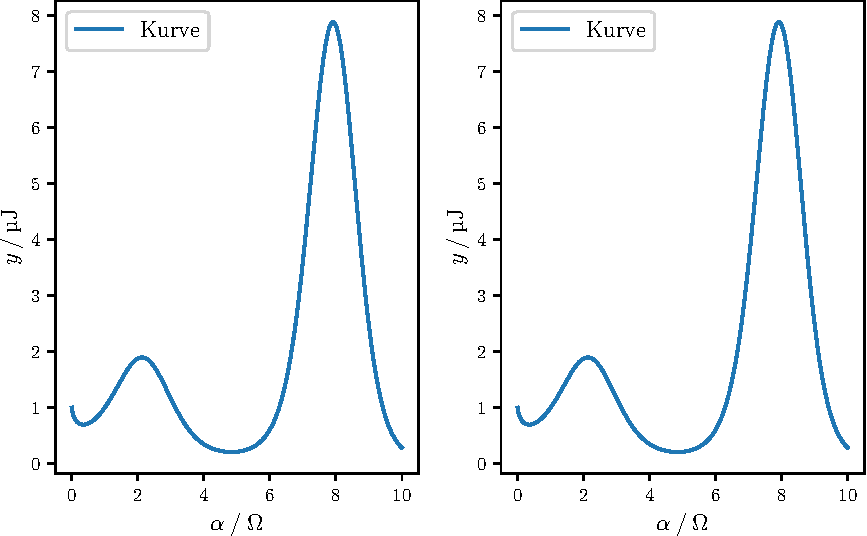
\includegraphics{plot.pdf}
  \caption{Abgleich mit Theoriekurve}
  \label{fig:plot}
\end{figure}
Es fällt auf, dass die Messwerte immer mehr von der Theoriekurve abweichen, je weiter sie vom Minimum entfernt sind. Dies spricht für eine ungenaue Messung.
Weiterhin lässt sich die Abweichung um das Minimum herum durch einen relativ hohen Klirrfaktor erklären. Nichts desto trotz ist eine Ähnlichkeit zur Theoriekurve
feststellbar.
\\
Der Klirrfaktor bestimmt sich durch (). Dabei wird die Näherung verwendet, dass die Summe der Oberwellen nur von der zweiten Oberwelle abhängt. Dementsprechen werden
nur noch $U_1$ und $U_2$ benötigt. $U_1$ ist durch $2,75\,\unit{\volt}$ von $U_s$ bei $f_0$ gegeben. $U_2$ bestimmt sich aus() und $\Omega = 2$ zu
\begin{align*}
  U_2 &= \frac{0,71\,\unit{\volt}}{\sqrt{\frac{(2^2 -1)^2}{9((1-2^2)^2 +9\cdot2^2)}}}\\
 &= 4,76\,\unit{\volt}.
\end{align*}
Der Klirrfaktor ergibt sich dann zu
\begin{align*}
  k &= \frac{U_2}{U_1} = \frac{4,76\,\unit{\volt}}{2,75\,\unit{\volt}} \\
  &= 1,73.
\end{align*}